\chapter{Use Case 1: Linear Algebra and Machine Learning}
\label{sec:lingebra}

In the first chapter, we have seen that within 
shared-memory parallel programming, we have broadly 
four options Confinement, Immutability, 
Use of Thread-safe Code, and Synchronization. 
More recently, we have seen four different  
implementations of a function called saxpy.
Let us continue exploring the options on the use 
case of linear algebra and machine learning. 

\section{Thread-safe Code in C++20}

\subsection{BLAS}

A key tool within linear algebra and machine learning are 
two ancient specifications, known as:
\begin{itemize} 
\item BLAS (``Basic Linear Algebra Subprograms''),
which covers vector addition, dot products, and linear combinations (this dates back to 1979).
 Level 2 added support for vector-matrix operations (1986),
 and level 3 added support for matrix-matrix operations and 
 block-partitioned algorithms (1988).
\item LAPACK (``Linear Algebra Package''), which 
covers matrix factorizations (LU, Cholesky and QR),
 eigenvalue and least squares solvers.
\end{itemize}

BLAS and LAPACK subroutines are all named naaop, where:
\begin{itemize} 
    \item n suggests whether to use real floating-point numbers in 
     single (S) or double (D) precision, 
     or complex number with single (C)
     or double (Z) precision.
    \item aa denotes the assumptions on the matrix, e.g., 
    diagonal (DI) specified by a vector, and 
    general matrix (GE).
    \item op denotes the algorithm, e.g., 
    matrix-matrix multiplication (MM), and 
    solving linear system (SV).
\end{itemize}
SGEMM is thus matrix-matrix multiplication of general dense matrices in single precision,
and DDOT is vector-vector dot product in double precision.
See Figure~\ref{blas02png} for an overview. 

\begin{figure}[t!]
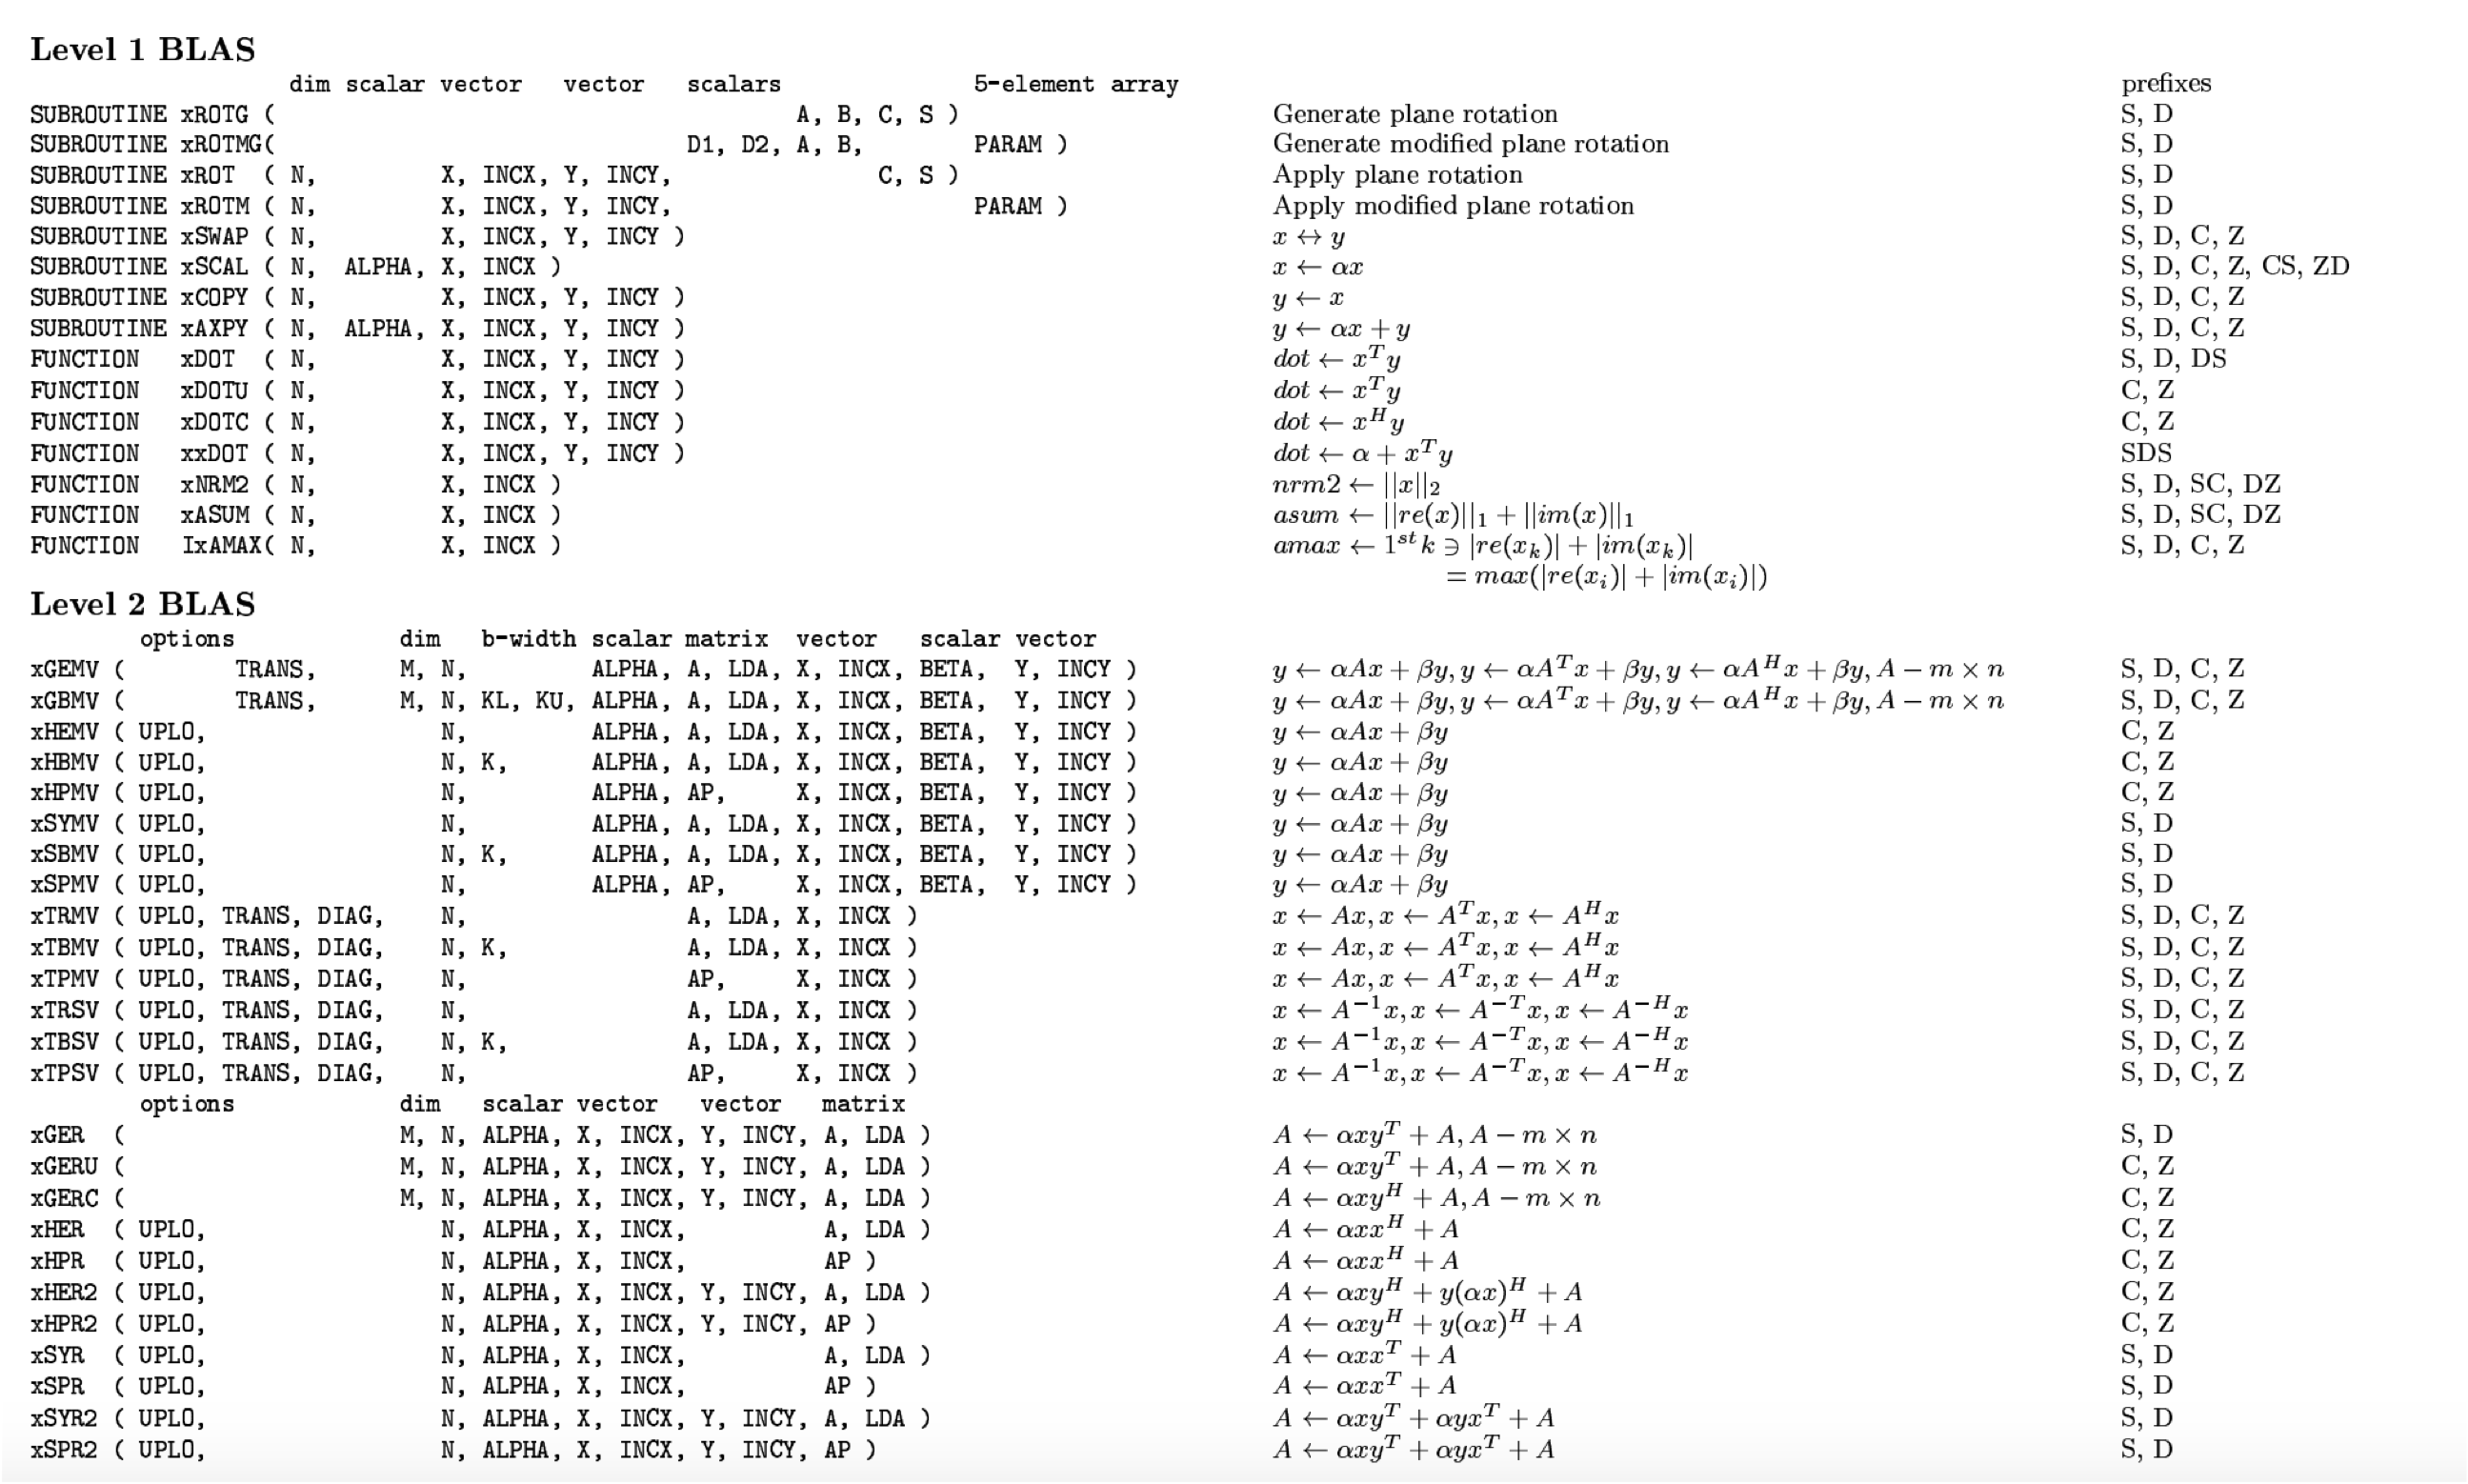
\includegraphics[width=\textwidth]{./static/blas02.png}
\caption{A summary of the routines in BLAS levels 1 and 2, from the cheat sheet \url{http://www.netlib.org/blas/blasqr.pdf
}.}
\label{blas02png}
\end{figure}

Most vendors of acclerators maintain their own BLAS 
 implementation:
 AMD maintains rocBLAS,
 Apple maintains Accelerate, 
 ARM maintains Arm Performance Libraries,
 Intel develops Intel Math Kernel Library (iMKL), and 
 NVIDIA maintains cuBLAS and NVBLAS.
Most libraries within linear algebra and machine learning
 supply BLAS user interface command structures, 
 which makes it easy to transfer the code.

Notable open-source implementation focussing 
mostly on CPUs are ATLAS, BLIS (BLAS-like Library Instantiation Software), and OpenBLAS.
A special mention should be devoted to the ATLAS library, 
which automatically optimizes itself for any architecture,
including complicated cache hierarchies. 

In turn, many further libraries and toolboxes are built 
around BLAS, including MATLAB, Mathematica, NumPy, R, 
and Julia.

\subsection{BLAS and C++}

For C++ , there are multiple implementations of BLAS, loosely speaking.
Libraries such as Armadillo, eigen, Intel OneAPI, LAPACK++, uBlas are 
sometimes linked against ancient Fortran code, but provide decent C++ interfaces. 
eigen and CLBlast actually provide C++ implementations too.

Intel OneAPI Mathematical Kernels comes with excellent documentation, 
examples, and support, but rather cumbersome naming conventions:

\begin{figure}[t!]
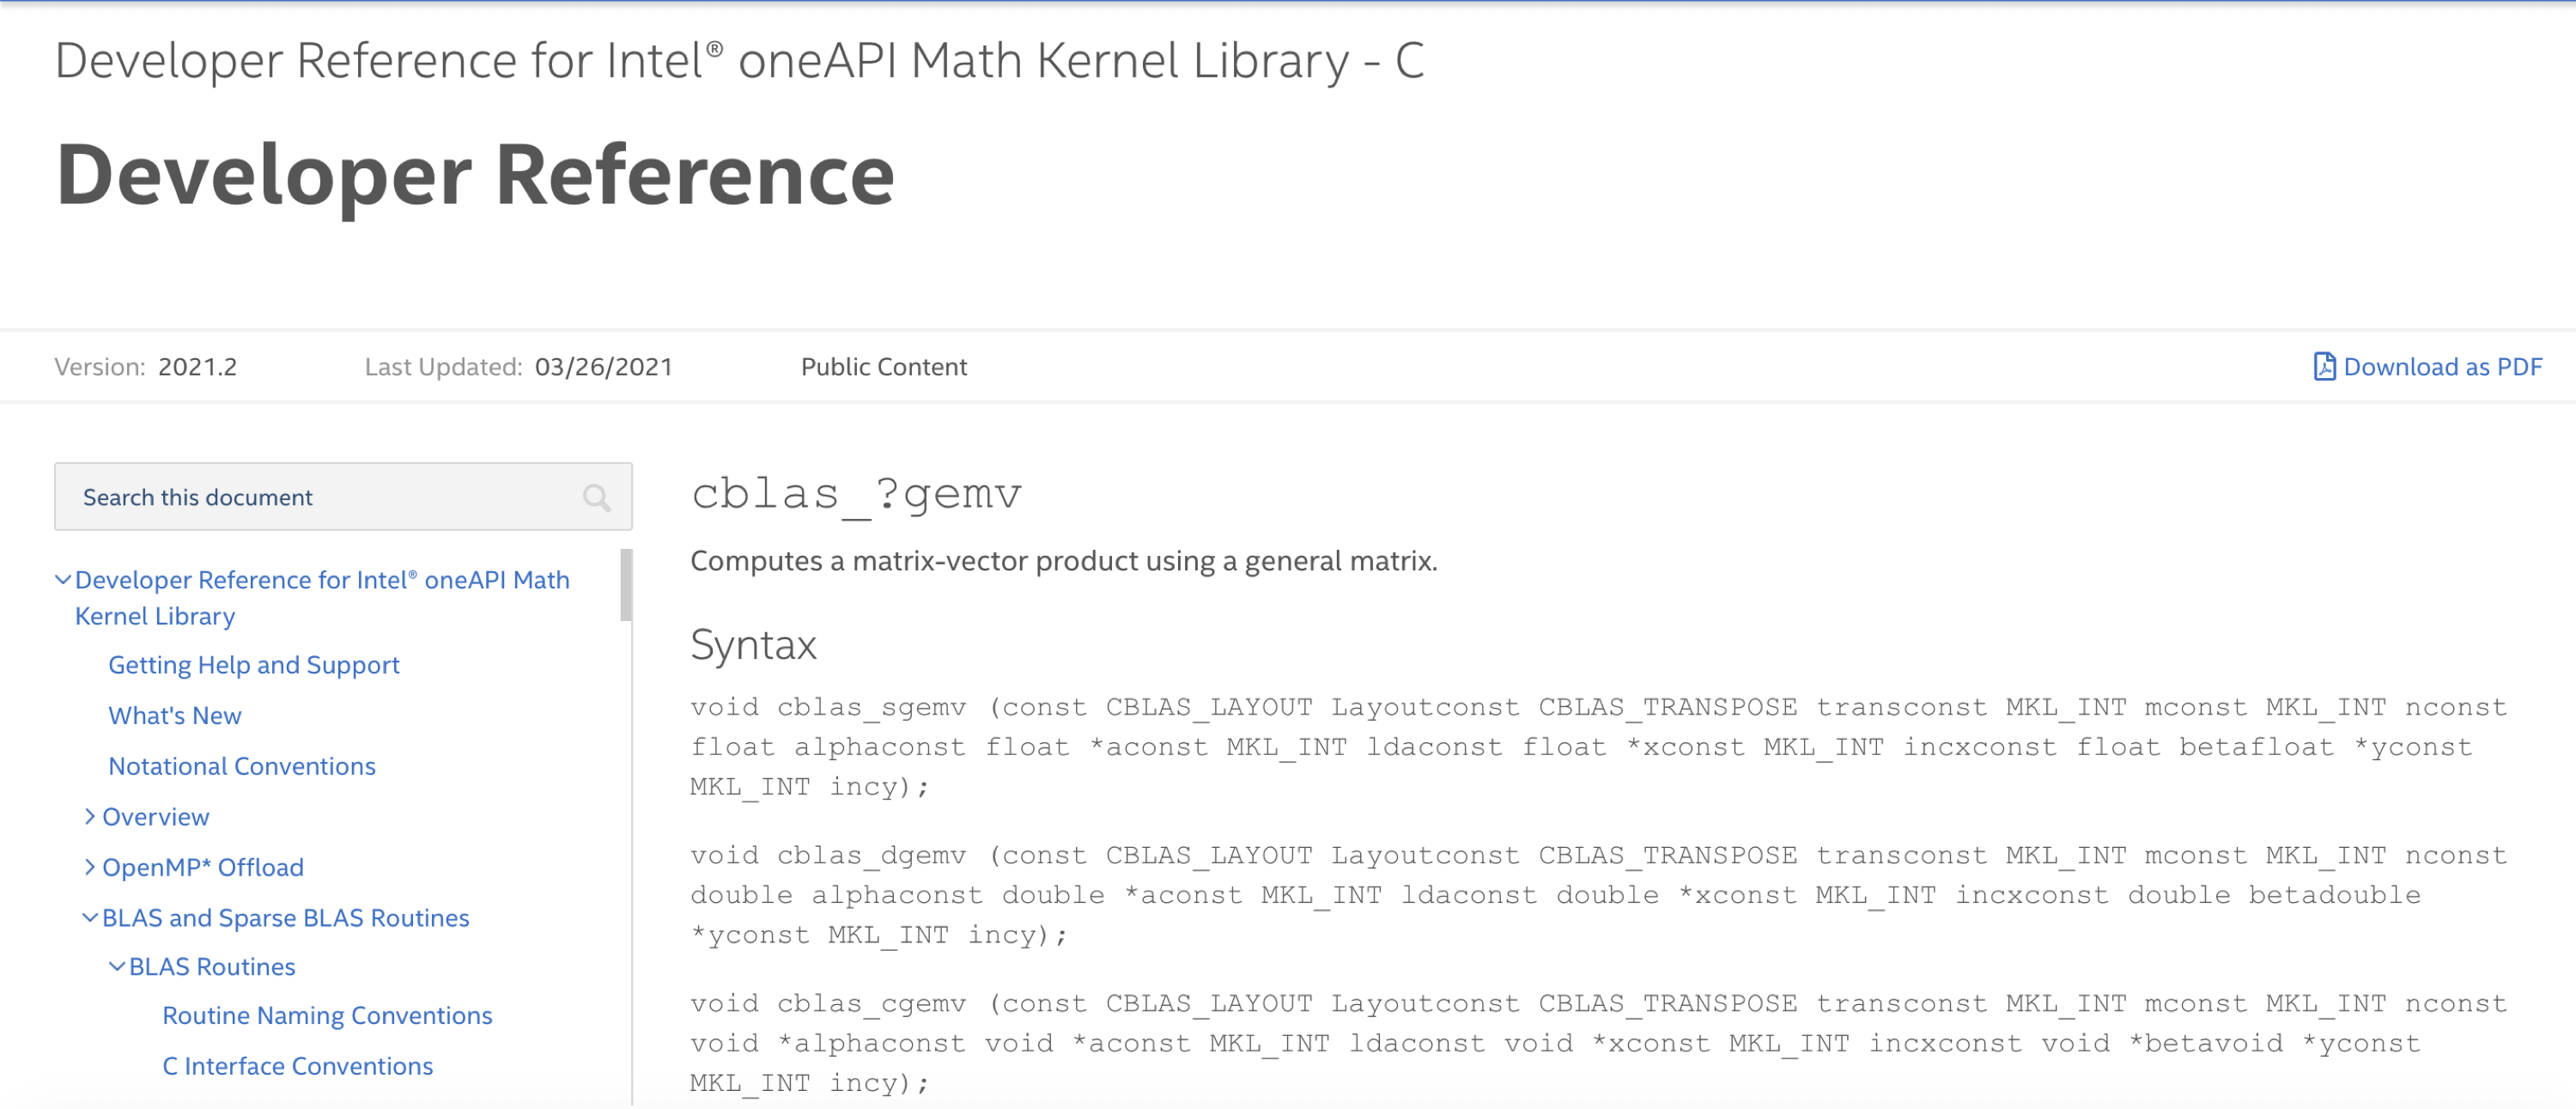
\includegraphics[width=\textwidth]{./static/blas01.png}
\caption{A screenshot from Intel OneAPI Mathematical Kernels.}
\label{blas01png}
\end{figure}

\begin{codebox}[breakable]{}
\footnotesize Example of the use of BLAS in C++ via Intel OneAPI.
\tcblower
\cppfile{code_examples/ml/blas01.cpp}
\end{codebox}

Boost.org uBlas provides a much more modern C++20-only syntax,
and can be linked to arbitrary vendor-provided BLAS library.
The example above could be rewritten, e.g., as:

\begin{codebox}[breakable]{}
    \footnotesize Example of the use of BLAS in C++ via Boost.org uBlas.
    \tcblower
    \cppfile{code_examples/ml/blas02.cpp}
\end{codebox}

As is clear from the preceding example, one can extend this well beyond matrices:

\begin{codebox}[breakable]{}
        \footnotesize A more elaborate example of the use of BLAS in C++ via Boost.org uBlas.
        \tcblower
        \cppfile{code_examples/ml/blas03.cpp}
\end{codebox}

\subsection{Scaling to Supercomputers}

As you may know, the tensor computations underlie much of modern machine learning,
in the form of training deep neural networks. 
The TensorFlow and PyTorch are key contenders there, 
again easy to link against any vendor-provided BLAS. 

Libraries such as TensorFlow make make it possible to
exploit much of the theoretically available processing 
power. See, for example, the plots 
in Figure \ref{fig:summit-tensorflow-performance2} and 
many further plots at 
\url{https://code.ornl.gov/olcf-analytics/summit/distributed-deep-learning-examples}.
This concerns the scaling of a code for training ResNet deep neural network on ImageNet 
benchmark on a supercomputer at the Oak Ridge National Laboratory 
in Tennessee, USA. 
The supercomputer has 
9,216 POWER9 22-core CPUs and 
27,648 NVIDIA Tesla V100 GPUs, each of which has 
5,120 CUDA Cores. 
In total, this means 141,557,760 cores with circa
200 petaFLOPS performance.
With a substantial amount of engineering and 
auto-tuning (using Horovod, cf. \cite{8945109}), one can achieve
near-linear scaling of performance (in terms of numbers of images trained per second) 
as a function of the number of cores. 
This, effectively, renders implementations 
``from scratch'' unnecessary. 

\begin{figure}[t!]
    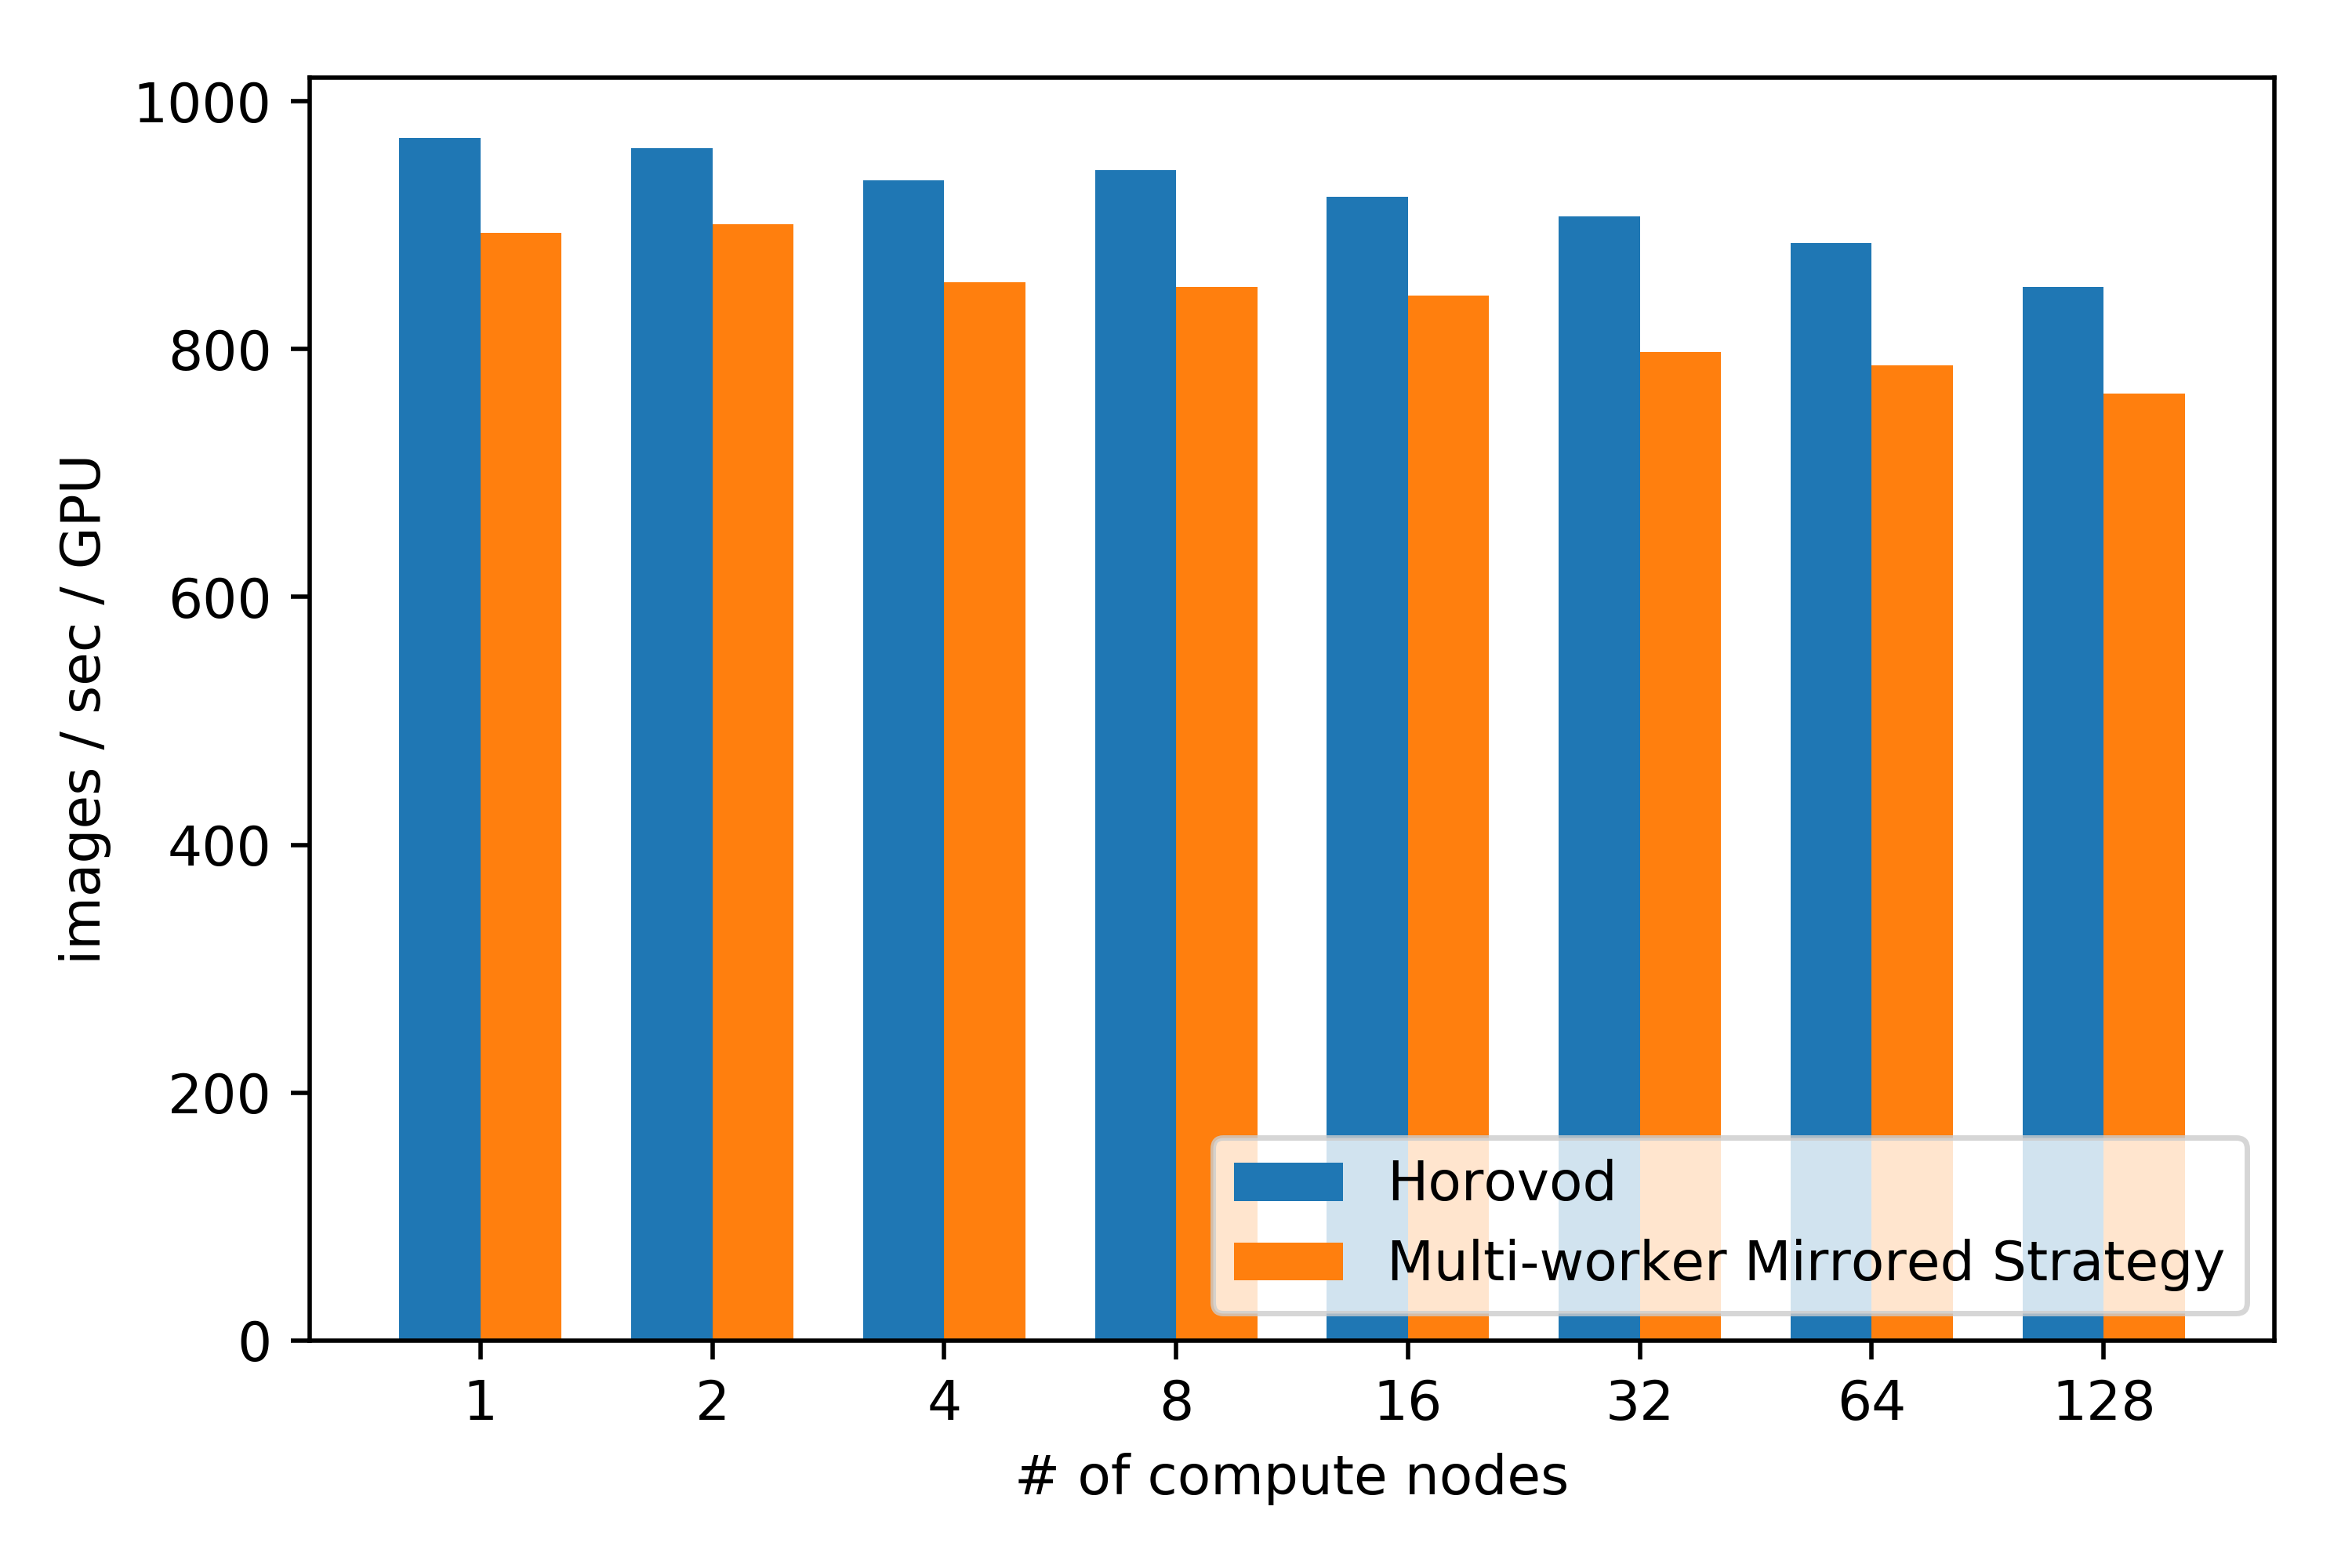
\includegraphics[width=\textwidth]{./static/summit-tensorflow-performance2.png}
    \caption{A summary of scaling of training ResNet on ImageNet in TensorFlow on Summit.}
    \label{fig:summit-tensorflow-performance2}
    \end{figure}

\section{Synchronization}

While it is very hard to see why one would like to 
implement one's own replacement of BLAS or LAPACK, it is
instructive to see several steps of the development
of common linear-algebraic routines. 
Let us explore matrix-matrix multiplication and 
solving of linear systems, as two examples. 

\subsection{Matrix-Vector Multiplication}

% TODO: Redo examples in SYCL as well!

Matrix-vector multiplication is a key primitive throughout 
linear algebra. Considering that the computation:
\begin{align}
    y_j= \sum_{i} a_{ji} x_i
\end{align}
for each coordinate $j$ in the resulting vector $y$,
can be computed in parallel, independently of any other,
it is almost embarrassingly (data) parallel. Still,
there are several important improvements over the basic version:  

\begin{codebox}[breakable]{}
\footnotesize An example of matrix multiplication in OpenMP.
\tcblower
\cppfile{code_examples/ml/multiply01_openmp.h}
\end{codebox}

Notably, one could aim to parallelize the processing of each row
of the matrix. This is difficult, due to the need for synchronization
in the addition into the result. 
One option would be to consider some auxiliary variable $z$,
which would be computed column-wise:

\begin{align}
z_{ij} = & a_{ij} x_j\\
y_i    = & \sum_{j} z_ij
\end{align}

This would be difficult, in terms of the cache hierarchies. 
We could, however, reorder the memory:

\begin{codebox}[breakable]{}
\footnotesize An example of matrix multiplication in OpenMP.
\tcblower
\cppfile{code_examples/ml/multiply02_openmp.h}
\end{codebox}

Alternatively, one can use the single most useful 
and embarrassingly simple trick of parallel programming:
introducing local variable. 

\begin{codebox}[breakable]{}
\footnotesize An example of matrix multiplication in OpenMP.
\tcblower
\cppfile{code_examples/ml/multiply03_openmp.h}
\end{codebox}

\subsection{Matrix-Matrix Multiplication}

Matrix-matrix multiplication is, likewise, very common and to some extent 
embarrassingly parallel. For large-enough matrices, the trivial parallelization
leads to too many small(ish) tasks. 

\begin{codebox}[breakable]{}
\footnotesize An example of matrix multiplication in OpenMP.
\tcblower
\cppfile{code_examples/ml/multiply04_openmp.h}
\end{codebox}

A more elaborate version considers blocking. This is actually very 
close to the state of the art algorithms:

\begin{codebox}[breakable]{}
\footnotesize An example of matrix multiplication in OpenMP.
\tcblower
\cppfile{code_examples/ml/multiply05_openmp.h}
\end{codebox}

%\begin{codebox}[breakable]{}
%\footnotesize An example of matrix multiplication in OpenMP.
%\tcblower
%\cppfile{code_examples/ml/multiply06_openmp.h}
%\end{codebox}

\subsection{Solving Linear Systems}

In commonly-known approaches to solving linear systems, 
the parallelization is less trivial. For example in Gauss
elimination, once you pick a pivot, a large submatrix 
(whose size depends on the pivot) needs to change. 
See for example:

\begin{codebox}[breakable]{}
\footnotesize An example of Gauss in OpenMP.
\tcblower
\cppfile{code_examples/ml/gauss01_openmp.h}
\end{codebox}

Notice, however, that one can rephrase the solving of 
a linear system in terms of solving a least squares
problem (minimizing the residual) and that modern 
optimization methods are competitive with tailor-made 
solvers for linear systems cf. \cite{gower2015randomized}.
One can hence focus on parallelizing optimization methods.
 

\subsection{Optimization for Machine Learning}

Much of machine learning is embarassingly parallel, 
incl. hyperparameter search, 
or data processing in Computer Vision, 
where one often has to process  
several streams of video in parallel, 
and sometimes can process several images or frames 
of a video in parallel.

Much else in machine learning is actually optimization,
which can be parallelized efficiently, 
either in coordinate descent methods,
or via stochastic gradient methods. 

For one example of such embarrassingly parallel computation, see 
\cite{akhriev2018pursuit}, which was originally developed 
for monitoring data from a city-wide camera network of a European capital. 
In one version of the code, similar to the snippet at  \url{https://github.com/jmarecek/OnlineLowRank},
the goal was to speed up the computation per single stream of video, such that each core handles one stream from a 4K camera in real-time. 

For another example of parallel programming in machine learning, see
\cite{marevcek2015distributed}, and the corresponding code at:
\url{https://github.com/optml/ac-dc/blob/master/cpp/src/solver/matrixCompletion/parallel/parallel_mc_opemmp.h}.

